\PassOptionsToPackage{quiet}{fontspec}
\documentclass{article}
\usepackage[UTF8]{ctex}
% Language setting
% Replace `english' with e.g. `spanish' to change the document language
\usepackage[english]{babel}

% Set page size and margins
% Replace `letterpaper' with`a4paper' for UK/EU standard size
\usepackage[letterpaper,top=2cm,bottom=2cm,left=3cm,right=3cm,marginparwidth=1.75cm]{geometry}

% Useful packages
\usepackage{amsmath}
\usepackage{graphicx}
\usepackage[colorlinks=true, allcolors=black]{hyperref}
\usepackage{amssymb}
\usepackage{titletoc}
\usepackage{titlesec}
\usepackage{fontspec}
\setmainfont{Times New Roman}
\usepackage{subfigure}
\usepackage{tikz}
\usetikzlibrary{positioning,petri}
\usetikzlibrary{arrows.meta,arrows,shapes,automata,backgrounds,petri,patterns,decorations.pathmorphing,positioning,calc,shapes.geometric}%插件
\usepackage{xcolor}
\usepackage{tcolorbox}
\usepackage{algorithmic}
\usepackage{diagbox}
\usepackage[ruled,vlined,linesnumbered]{algorithm2e}
\usepackage{tabu}
\usepackage{multirow}
\usepackage{booktabs}
\usepackage{framed}
\usepackage{hyperref}

\RequirePackage{xeCJK} 
\setCJKfamilyfont{KaiTi}{KaiTi} \newcommand{\song}{\CJKfamily{KaiTi}}


\hypersetup{
    colorlinks=true,
    linkcolor=black,
    filecolor=magenta,      
    urlcolor=blue,
    pdftitle={Overleaf Example},
    pdfpagemode=FullScreen,
    }







\titleformat{\section}{\normalfont\Large\bfseries}{\thesection.}{0.2em}{}
\titleformat{\subsection}{\normalfont\large\bfseries}{\thesubsection}{0.2em}{}

\newtheorem{definition}{Definition}
\newtheorem{example}{Example}
\newtheorem{problem}{Problem}
\newtheorem{remark}{Remark}
\newtheorem{derivation}{Derivation}
\newtheorem{proposition}{Proposition}




\begin{document}




\title{
\includegraphics[width=1.2in]{MUST.png}\\[-2pt]\huge Macau University of Science and Technology
~\\
Faculty of Innovation Engineering
~\\
Dept. of Engineering Science
~\\
\LARGE{(澳門科技大學創新工程學院工程科學系)}
~\\[40pt]

Thesis Proposal 
~\\
(論文選題報告)
~\\[40pt]

\textbf{\LARGE Title}

\title{}

~\\[50pt]





\large{

 Submitted by: 王茗琛 

~\\[1pt]

 Student No.: 2230025907 

~\\[1pt]

 Supervisor: 劉新} 
 
     } 

\author{}

\date{}


\titlecontents{section}[0pt]{\addvspace{5pt}\filright}              
{\contentspush{\thecontentslabel\ 
}}              
{}{\titlerule*[8pt]{.}\contentspage}


\maketitle
\thispagestyle{empty}

\clearpage




\pagenumbering{roman}
\renewcommand{\abstractname}{\Large Abstract\\}
\begin{abstract}
This research deals with the supervisory control problem of discrete event systems. Use singular keywords. Keywords are separated by commas or semicolons, and there is often a period at the end.


The template can be used in online and offline ways. For the former (highly recommended), 
Overleaf (\url{https://www.overleaf.com}) is a collaborative cloud-based LaTeX editor used for writing, editing and publishing scientific documents, which is much easy to use and friendly.

For the latter, one can use Texstudio, which is a very popular yet free software package (\url{https://www.texstudio.org/}). When using Texstudio, the compiling command is \textcolor{blue}{XeLatex}. To make Texstudio work, one need to first install \textcolor{blue}{Miktex}, see \url{https://miktex.org/}. We happen to find, rather rarely, that a successful compiling may depend on the version of Texstudio. In any case, we recommend the latest version of Texstudio.


\textbf{keywords}: Discrete event system; supervisory control; fault diagnosis.
\end{abstract}

\phantomsection\addcontentsline{toc}{section}{Abstract}\tolerance=500



\newpage


\clearpage

\renewcommand{\abstractname}{\Large 摘要\\}
\begin{abstract}
\medskip


中文摘要一般300到500字且使用繁體. 使用西文方式下的標點符號. 比如, 像這樣. 若對模板使用有任何問題, 可email至 \href{mailto:zhwli@ieee.org}{zhwli@ieee.org}.

\medskip
\textbf{關鍵詞}:一般使用3--5個關鍵詞,中間用分號隔開. 
\end{abstract}

\phantomsection\addcontentsline{toc}{section}{摘要}\tolerance=500

\newpage



\ctexset{ contentsname = {Table of Contents}}

\tableofcontents  

   \phantomsection\addcontentsline{toc}{section}{Table of Contents}\tolerance=500
\newpage

\pagenumbering{arabic}
\setcounter{page}{1}

\section{Introduction}
\subsection{Research Background}

xxxxxx.

Fang develops a method for supervisor synthesis ... \cite{Fang2019}.







\subsection{Motivation}

xxxxxx.



\subsection{Research Objectives}

xxxxxx.




\section{Literature Review}

xxxxxx.

We give some examples of how to draw figures.

\begin{figure}[htbp]
\begin{center}
	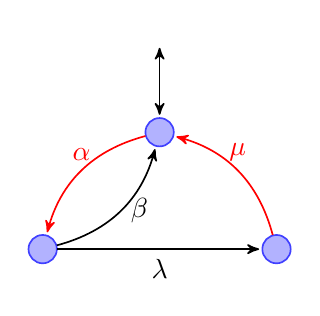
\begin{tikzpicture}
				[->,>=stealth',shorten >=1pt,auto,node distance=3.5cm,
				semithick,scale=.6,bend angle=45]
				%%%右箭头,箭头样式,自动适应,node默认间距,线条默认半粗,比例,默认弯角
				\tikzstyle{every state}=[fill=blue!30,draw=blue!75,text=black,minimum size=6mm,scale=1.5]
				%默认state样式为蓝色(0-100)填充,蓝色线条,黑色文本,最小size,比例
				%画出所有node
				\node[state,scale=0.4](0)                       {};
				%大括号内是node中的内容,(0)为该node的代号
				\node[state,scale=0.4](1) [below left of=0]     {};
				%[]内为(1)在(0)的左下位置,默认间距
				\node[state,scale=0.4](2) [below right of=0]    {};
				\node[draw=white]at(90:2)                       {}
				%一个不画出的node,由角坐标给出位置,注意这里还没有分号
				edge[<->](0);%其后可以直接定义edge,以分号结束指令
				
				
				%在node之间添加连线.第一个中括号中内容是连线的性质(颜色、弯曲方向和角度)
				%第二个括号中的内容是每条连线所附带的字母与连线的相对位置。有right\left\below\above可选
				\path 
				(0)edge [red,bend angle=30,bend right]node[above]{$\alpha$}      (1) %0到1
				(1)edge [bend angle=30,bend right]    node[right]{$\beta$}       (0)  
				(1)edge                               node[below]{$\lambda$}     (2)
				(2)edge [red,bend angle=30,bend right]node[above]{$\mu$}         (0)
				;%完整指令后以分号结束
			\end{tikzpicture}
\end{center}
\caption{This is an automaton.}
    \label{fig:my_label}
\end{figure}

\begin{figure}[htbp]
\centering
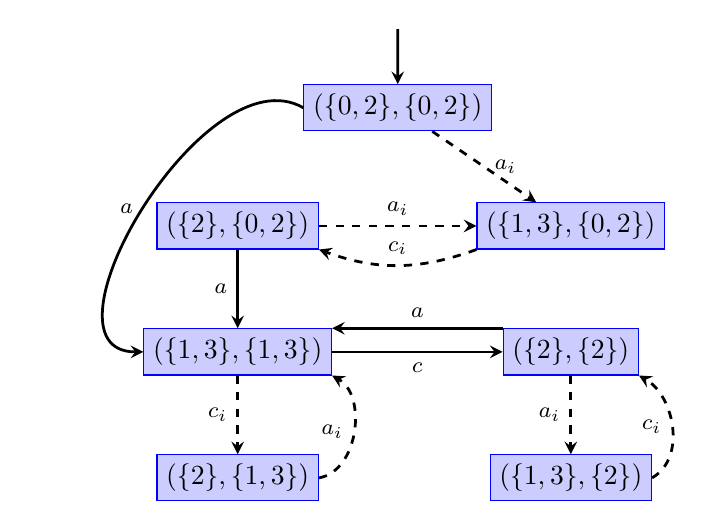
\begin{tikzpicture}[>=stealth]
	\node (state0) [draw=blue,fill=blue!20,xshift=2cm] {$(\{0,2\},\{0,2\})$};
	\node (state1) [draw=blue,fill=blue!20,left=1cm of state0.center,yshift=-1.5cm] {$(\{2\},\{0,2\})$};
    \node (state2) [draw=blue,fill=blue!20,right=1cm of state0.center,yshift=-1.5cm] {$(\{1,3\},\{0,2\})$};
    \node (state3) [draw=blue,fill=blue!20,below=1.3cm of state1.center] {$(\{1,3\},\{1,3\})$};
    \node (state4) [draw=blue,fill=blue!20,below=1.3cm of state2.center] {$(\{2\},\{2\})$};
    \node (state5) [draw=blue,fill=blue!20,below=1.3cm of state3.center] {$(\{2\},\{1,3\})$};
    \node (state6) [draw=blue,fill=blue!20,below=1.3cm of state4.center] {$(\{1,3\},\{2\})$};
    \draw[->,line width=1pt]  (2,1) -- (state0.north);
    \draw [->,line width=1pt,dashed] (state0) to node [right] {\footnotesize$a_{i}$} (state2);
	\draw [->,line width=1pt,dashed] (state1) to node [above] {\footnotesize$a_{i}$} (state2);
    \draw [->,line width=1pt,dashed] (state2.south west) to [in=340,out=200] node [above] {\footnotesize$c_{i}$} (state1.south east);
    \draw [->,line width=1pt,dashed] (state3.south) to node [left] {\footnotesize$c_{i}$} (state5.north);
	\draw [->,line width=1pt,dashed] (state5.east) to [in=330,out=10] node [left] {\footnotesize$a_{i}$} (state3.south east);
    \draw [->,line width=1pt,dashed] (state4.south) to  node [left] {\footnotesize$a_{i}$} (state6.north);
    \draw [->,line width=1pt,dashed] (state6.east) to [in=330,out=30] node [left] {\footnotesize$c_{i}$} (state4.south east);
    \draw [->,line width=1pt] (state1) to node [left] {\footnotesize$a$} (state3);
    \draw [->,line width=1pt] (state3) to node [below] {\footnotesize$c$} (state4);
    \draw [->,line width=1pt] (state4.north west) to node [above] {\footnotesize$a$} (state3.north east);
    \draw [->,line width=1pt] (state0.west) to [in=180,out=150] node [left] {\footnotesize$a$} (state3.west);
\end{tikzpicture}
\caption{Indicator automaton and verifier of the NFA in Fig. \ref{fig:my_label}}\label{indicator-NFA}
\end{figure}





\section{Xxxx (your research topic)}

\subsection{xxxxxx}

We give some examples of how to make tables.

The table title is at the top of the table.

\begin{table}[htbp]	
	\centering
	\caption{A table.}
	\begin{tabular}[l]{@{}lcccccc}		
		\toprule		
		Class$^{\rm a}$ & $\gamma_1$ & $\gamma_2$$^{\rm b}$& $\langle \gamma \rangle$& $G$ & $|{ f}|$ & $\theta _{c}$ \\		
		\midrule	
		BL Lacs &5 & 36 & 7 & $-4.0$ & $1.0\times 10^{-2}$ & 10$^\circ$ \\		
		FSRQs & 5 & 40 & 11 & $-2.3$ & $0.5\times 10^{-2}$ & 14$^\circ$ \\		
		\bottomrule		
	\end{tabular}
	\label{tab:t1}
\end{table}

\begin{table}[htbp]  
\caption{Another table.}  
\begin{center}  
\begin{tabu} to 0.8\textwidth{X[c]|X[3,b]|X[2,l]|X[c]|X[3,m]|X[1,c]}  
%0.8\textwidth   为设置表格宽度  
%X[c]      表示这一列居中,所占比例为1,相当于X[1,c]  
%X[3,c]   表示这一列居中,所占比例为3,这列的宽度是X[c]列的3倍  
\hline  
$i$  &$x_i$              &$n_i$      &$i$    &$x_i$               &$n_i$\\  
\hline  
1    &0.5$\sim$0.64       &1           &8    &1.48$\sim$1.62      &53\\  
2    &0.64$\sim$0.78      &2           &9    &1.62$\sim$1.76      &25\\  
3    &0.78$\sim$0.92      &9           &10   &1.76$\sim$1.90      &19\\  
4    &0.92$\sim$1.06      &26          &11   &1.90$\sim$2.04      &16\\  
5    &1.06$\sim$1.20      &37          &12   &2.04$\sim$2.18      &3\\  
6    &1.20$\sim$1.34      &53          &13   &2.18$\sim$2.38      &1\\  
7    &1.34$\sim$1.48      &56          &     &                    & \\  
\hline  
\end{tabu}  
\end{center}  
\end{table}



\subsection{xxxxxx}

xxxxxx.

Formal expression is very important.

Example 1:
\begin{equation}
\label{eq1}
	e^{\pi i}+1=0
\end{equation}

Example 2:
\begin{equation}
\label{eq2}
	a^2+b^2=c^2
\end{equation}

If no equation number is needed, we can use double dollars at the beginning and end of the equation.

$$
\cos{x}+\sin{y}=1.
$$

Example 3:
\begin{equation}
\label{eq3}
\quad\dbinom{n}{m}=\dbinom{n}{n-m}=C_n^m=C_n^{n-m}
\end{equation}

Example 4:
\begin{equation}
    (a + b)^3 = (a + b) (a + b)^2=a^3 + 3a^2b + 3ab^2 + b^3     
\end{equation}

Here are more examples of mathematics equations or expression.


\begin{equation}
  x = a_0 + \cfrac{1}{a_1 
          + \cfrac{1}{a_2 
          + \cfrac{1}{a_3 + \cfrac{1}{a_4} } } }
\end{equation}




\begin{equation*}
\frac{
    \begin{array}[b]{r}
      \left( x_1 x_2 \right)\\
      \times \left( x'_1 x'_2 \right)
    \end{array}
  }{
    \left( y_1y_2y_3y_4 \right)
  }
\end{equation*}


\[
P\left(A=2\middle|\frac{A^2}{B}>4\right)
\]


\[
M = \begin{bmatrix}
       \frac{5}{6} & \frac{1}{6} & 0           \\[0.3em]
       \frac{5}{6} & 0           & \frac{1}{6} \\[0.3em]
       0           & \frac{5}{6} & \frac{1}{6}
     \end{bmatrix}
\]


\[
M = \bordermatrix{~ & x & y \cr
                  A & 1 & 0 \cr
                  B & 0 & 1 \cr}
\]


\[ f(n) =
  \begin{cases}
    n/2       & \quad \text{if } n \text{ is even}\\
    -(n+1)/2  & \quad \text{if } n \text{ is odd}
  \end{cases}
\]



\[
\left(
    \begin{array}{c}
      n \\
      r
    \end{array}
  \right) = \frac{n!}{r!(n-r)!}
\]



Here are some logic expressions:


$$
(\forall s\in\overline{K})(\forall\sigma\in\Sigma)(\forall s^\prime\in\overline{K})s\sigma\in L(G)~\&~s^\prime\sigma\in L(G)~\&~Ps=Ps^\prime\implies s^
\prime\in\overline{K}.
$$




For more details about mathematics equations or expressions, see \url{https://en.wikibooks.org/wiki/LaTeX/Mathematics}.

\section{XXXX (another topic if necessary)}

\subsection{Algorithm}

An example of the Algorithm 1.


\begin{algorithm} 
	\SetAlgoVlined 
	\caption{Control policy construction} 
	\KwIn{Control parameter $r_i$, time series $Backgrd(T_i)$=${T_1,T_2,\ldots, T_n}$ and similarity threshold $\theta_r$} 
	\KwOut{Control policy $con(r_i)$} 
	$con(r_i)= \Phi$\; 
	\For{$j=1; j \le n; j \ne i$} 
	{ 
		float $maxSim=0$\; 
		$r^{maxSim}=null$\; 
		\While{not end of $T_j$} 
		{ 
			compute Jaro($r_i,r_m$);~~ \% here are the commentary texts 

		} 
		$con(r_i)=con(r_i)\cup {r^{maxSim}}$\; 
	} 
	return $con(r_i)$\; 
\end{algorithm}


\subsection{xxxx}
\subsubsection{xxxx}





\section{Schedule for the thesis}





\section{Publications}



\newpage
\phantomsection\addcontentsline{toc}{section}{References}\tolerance=500

\begin{thebibliography}{10}

	\bibitem{WOS:000441446300034}
		C. Y.~Yin, J. W.~Xi, R. X.~Sun and J.~Wang, ``Location privacy protection based on
		differential privacy strategy for big data in industrial internet of
		things,'' \emph{IEEE Transactions on Industrial Informatics}, vol.~14, no.~8,
		pp. 3628--3636, Aug. 2018.
		
		\begin{framed}	
		\textcolor{blue}{For a paper in a journal, the title of the journal should be in Italics. The first letter of each word should be capitalized. Volume and Issue numbers should be given. There is a blank space between ``vol'' and ``14'' in the above. Note that two continuous hyphens in $\text{\LaTeX}$ generates ``--''.  }
		\end{framed}
		
		\bibitem{WOS:000526381800058}
		J. B.~Xiong, R.~Ma, L.~Chen, Y. L.~Tian, Q.~Li, X. M.~Liu and Z. Q.~Yao, ``A personalized
		privacy protection framework for mobile crowdsensing in IIoT,'' \emph{IEEE
			Transactions on Industrial Informatics}, vol.~16, no.~6, pp. 4231--4241, Jun.
		2020.
		
		
		\bibitem{WOS:000333098100011}
		R.~De~Prisco and A.~De~Santis, ``On the relation of random grid and
		deterministic visual cryptography,'' \emph{IEEE Transactions on Information
			Forensics and Security}, vol.~9, no.~4, pp. 653--665, Apr. 2014.
		
		\bibitem{WOS:000391501000014}
		M.~Beunardeau, A.~Connolly, R.~Geraud and D.~Naccache, ``White-box
		cryptography: Security in an insecure environment,'' \emph{IEEE Security and
			Privacy}, vol.~14, no.~5, pp. 88--92, Sep. 2016.
		
		\bibitem{WOS:000179217500008}
		L.~Sweeney, ``K-anonymity: A model for protecting privacy,''
		\emph{International Journal of Uncertainty, Fuzziness and Knowledge-Based
			Systems}, vol.~10, no.~5, pp. 557--570, Oct. 2002.
		
		\bibitem{WOS:000324313400046}
		P. S.~Wang and J. D.~Wang, ``L-diversity algorithm for incremental data release,''
		\emph{Applied Mathematics and Information Sciences}, vol.~7, no.~5, pp.
		2055--2060, Sep. 2013.
		
		\bibitem{WOS:000217109300002}
		S.~Ruggieri, ``Using t-closeness anonymity to control for non-discrimination,''
		\emph{Transactions on Data Privacy}, vol.~7, no.~2, pp.
		99--129, Aug. 2014.
		
		\bibitem{WOS:000265070900029}
		C.~Dwork, ``The differential privacy frontier (extended abstract),'' in
		\emph{Proc. 6th Theory of Cryptography Conference}, vol. 5444, pp. 496--502, Mar. 2009.
		
			\begin{framed}	
		\textcolor{blue}{For a paper in conference proceedings, the name of the conference should be in Italics. The first letter of each word should be capitalized. Note that before ``\emph{Proc.}'', there is a word ``in'' that is not in Italics.}
		\end{framed}
		
		\bibitem{WOS:000255239500001}
		C.~Dwork, ``Differential privacy: A survey of results,'' in \emph{Proc. 5th International Conference on Theory and Applications of Models of Computation}, vol.
		4978, pp. 1--19, Apr. 2008.
		
		\bibitem{WOS:000268182000042}
		C.~Dwork and J.~Lei, ``Differential privacy and robust statistics,'' in
		\emph{Proc. 41st Annual ACM Symposium on Theory of Computing}, pp. 371--380, May. 2009.
		
		\bibitem{WOS:000236909300014}
		C.~Dwork, F.~McSherry, K.~Nissim and A.~Smith, ``Calibrating noise to
		sensitivity in private data analysis,'' in \emph{Proc. 3rd Theory of Cryptography Conference}, vol. 3876, pp. 265--284, Mar. 2006.
		
		\bibitem{WOS:000252161900009}
		F.~McSherry and K.~Talwar, ``Mechanism design via differential privacy,'' in
		\emph{Proc. 48th Annual IEEE Symposium on Foundations of Computer Science}, pp. 94--103, Oct. 2007.
		
		\bibitem{WOS:000409749800001}
		C.~Dwork and A.~Roth, ``The algorithmic foundations of differential privacy,''
		\emph{Foundations and Trends in Theoretical Computer Science}, vol.~9, no. 3, pp. 211--406, Jan. 2013.
		
		\bibitem{WOS:000365190400003}
		C.~Li, G.~Miklau, M.~Hay, A.~McGregor and V.~Rastogi, ``The matrix mechanism:
		Optimizing linear counting queries under differential privacy,'' \emph{VLDB
			Journal}, vol.~24, no.~6, pp. 757--781, Dec. 2015.
		
		\bibitem{WOS:000369309900022}
		Q. Geng and P. Viswanath, ``The optimal noise-adding mechanism in differential privacy,'' \emph{IEEE Transactions on Information Theory}, vol.~62, no.~2, pp. 925--951, Feb. 2016.
		
	
		

		
		\bibitem{WOS:000214000900007}
		J.~W. Bryans, M.~Koutny and P.~Y.~A. Ryan, ``Modelling opacity using Petri
		nets,'' \emph{Electronic Notes in Theoretical Computer Science}, vol. 121,
		pp. 101--115, Feb. 2005.
		
	
	
		
		\bibitem{WOS:000388376100124}
		Y.~Tong, Z. Y.~Ma, Z. W.~Li, C.~Seatzu and A.~Giua, ``Verification of language-based
		opacity in Petri nets using verifier,'' in \emph{Proc. American Control Conference (ACC)}, pp. 757--763, Jul. 2016.
		
	
		
		
		\bibitem{WOS:000079708900643}
		R.~Kumar and V. K.~Garg, ``Control of stochastic discrete event systems: Synthesis,'' in \emph{Proc. 37th IEEE Conference on Decision and Control}, pp. 3299--3304, Dec. 1998.
		
		\bibitem{WOS:000298615101112}
		Y. S. Huang and M.~Jeng, \emph{Fault Diagnosis of Discrete Event Systems: A Timed Automaton Approach}, Springer-verlag, Berlin, 2011.
		
		\begin{framed}	
		\textcolor{blue}{This is a book or monograph.  }
		\end{framed}

\bibitem{Fang2019}
~F. F. Fang, \emph{A Journey to the West}, Ph.D. Dissertation, Institute of Systems Engineering, Macau University of Science and Technology, July 2021.
2019.

\begin{framed}	
		\textcolor{blue}{This is a degree thesis.  }
		\end{framed}

  
  
\end{thebibliography}

\end{document}